%%%%%%%%%%%%%%%%%%%%%%%%%%%%%%%%%%%%%%%%%%%%%%%%%%%%%%%%
% Este é um documento que servirá de modelo para
% os relatórios feitos na disciplina Laboratório de Circuitos Lógicos
% 2020-2
%%%%%%%%%%%%%%%%%%%%%%%%%%%%%%%%%%%%%%%%%%%%%%%%%%%%%%%%%

%%%%%%%%%%%%%%%%%%%%%%%%%%%%%%%%%%%%%%%%%%%%%%%%%%%%%%%%%
% Use os diferentes diretórios para colocar os relatórios de cada experimento, deste modo vc consegue manter um histórico e todo material organizado em apenas um local.
% Lembre-se de mudar o Main Document no Menu!!!

\documentclass[12pt]{article}

\usepackage{sbc-template}
\usepackage[brazil,american]{babel}
\usepackage[utf8]{inputenc}

\usepackage{graphicx}
\usepackage{url}
\usepackage{float}
\usepackage{listings}
\usepackage{color}
\usepackage{todonotes}
\usepackage{algorithmic}
\usepackage{algorithm}
\usepackage{hyperref}
\usepackage{amsmath}
\usepackage{graphicx}
\usepackage{array}
\usepackage{mwe}
\usepackage[shortlabels]{enumitem}

\usepackage{xcolor}
\usepackage{listings}
\usepackage[electronic]{ifsym}
\definecolor{vgreen}{RGB}{104,180,104}
\definecolor{vblue}{RGB}{49,49,255}
\definecolor{vorange}{RGB}{255,143,102}

\lstdefinestyle{verilog-style}
{
    language=Verilog,
    basicstyle=\small\ttfamily,
    keywordstyle=\color{vblue},
    identifierstyle=\color{black},
    commentstyle=\color{vgreen},
    numbers=left,
    numberstyle=\tiny\color{black},
    numbersep=10pt,
    tabsize=8,
    moredelim=*[s][\colorIndex]{[}{]},
    literate=*{:}{:}1
}

\makeatletter
\newcommand*\@lbracket{[}
\newcommand*\@rbracket{]}
\newcommand*\@colon{:}
\newcommand*\colorIndex{%
    \edef\@temp{\the\lst@token}%
    \ifx\@temp\@lbracket \color{black}%
    \else\ifx\@temp\@rbracket \color{black}%
    \else\ifx\@temp\@colon \color{black}%
    \else \color{vorange}%
    \fi\fi\fi
}
\makeatother

\usepackage{trace}

\sloppy


\title{Experimento 9\\
Contadores Assíncronos e Síncronos}

\author{Matheus Cardoso de Souza, 202033507\\
        Ualiton Ventura da Silva, 202033580\\
        Grupo G42
}

%%%% LEMBRE-SE DE MUDAR O GRUPO NA LINHA ABAIXO!!!!! %%%%%%
\address{Dep. Ciência da Computação -- Universidade de Brasília (UnB)\\
  CIC0231 - Laboratório de Circuitos Lógicos
  \email{matheus-cardoso.mc@aluno.unb.br, 202033580@aluno.unb.br}
}

\begin{document}
\maketitle

\selectlanguage{american}
 \begin{abstract}
   \textbf{TODO}
 \end{abstract}

\selectlanguage{brazil}
 \begin{resumo}
   O presente relatório tem como objetivo a elaboração de contadores assíncronos
   e síncronos, sendo que para seu uso são utilizados flip-flops JK, através de
   sua elaboração também será analisado a propogação de erro existente ao
   associar-se flip-flops.
 \end{resumo}


\section{Introdução}\label{sec:Introducao}

Flip-flops no geral possuem diversos usos para a elaboração de sistemas
computacionais, sendo utilizados não somente para a criação de dispositivos de
memórias bem como para contadores, divisores de frequência dentre outras
aplicações.\\ \\
Tratando-se de contadores síncronos tem-se que sua característica como contador
refere-se ao mesmo clock para todos os flip-flops associados, assim a mudança
que ocorre nas bordas será simultânea para todos flip-flops
utilizados.[Referencia dos slides] \\ \\
Utilizando um flip-flop tipo T, este contador poderia ser expresso como:
\begin{figure}[H]
  \centering
  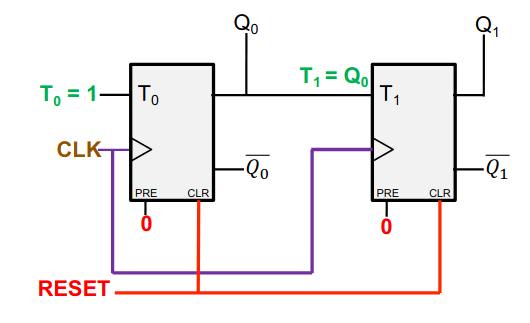
\includegraphics[width=0.5\textwidth]{Exp09/images/ContadorSincrono.png}
  \caption{Exemplo de Contador Síncrono de 2 bits}\label{fig:ContadorSincrono.png}
\end{figure}
% TODO: A referência é o slide de contador síncrono de CL
Detalhe a mencionar-se é o fato de que este contador somente é possível por a
existência de atrasos, pois, na borda de subida que registra mudança, tanto o
primeiro quanto segundo flip flop irão mudar, porém, o primeiro modifica-se
somente após a borda, assim o segundo irá possuir o estado anterior do primeiro.

Utilizando um contador assíncrono temos que a mudança de cada contador irá
ocorrer dependendo do anterior, assim, existem atrasos associados na mudança de
estado em um aspecto geral, sendo que este tipo de contador é descrito
utilizando flip-flops tipo T como:

\begin{figure}[H]
  \centering
  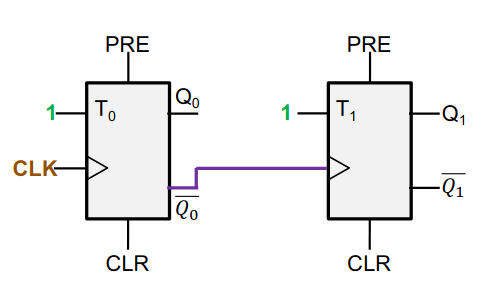
\includegraphics[width=0.5\textwidth]{Exp09/images/ContadorAssincrono.png}
  \caption{Exemplo de Contador Assíncrono de 2 bits}\label{fig:ContadorAssincrono.png}
\end{figure}

Cada um dos flip-flops utilizados possuem uma característica que tornam-os
necessários para determinados usos, por exemplo, um contador assíncrono por
possuir flip-flops que dependendem uns dos outros possui um atraso propagação
dos estados, assim, temos que a frequência de um flip-flop para o seu próximo
irá ser reduzida pela metade, portanto, contadores assíncronos podem ser
utilizados como divisores de frequência.

\subsection{Objetivos}\label{sec:Objetivos}

Através dos procedimentos realizados será observado de maneira geral uma análise
referente ao comportamento de contadores e seu funcionamento, para os
experimentos feitos será utilizado flip-flops do tipo T e JK, contudo, deve-se
mencionar que estes mesmos procedimentos poderiam ser feitos utilizando outros
tipos de flip-flops, por exemplo, flip-flops do tipo T podem ser expressos
através dos tipo D e assim inversamente.

\subsection{Materiais}\label{sec:Materiais}

Em função da natureza do ensino a distância, os presentes experimentos não foram
realizados usando-se materiais e equipamentos físicos, mas sim emulados por meio
do software
\href{https://www.digitalelectronicsdeeds.com/downloads.html}{Deeds}.

A seguir estão enumerados os materiais utilizados:
\begin{itemize}
    \item Software Deeds
    \item Portas lógicas
    \begin{itemize}
      \item \emph{NAND}s de $2$ entradas
      \item \emph{NOR}s de $2$ entradas
      \item \emph{Flip-flops JK-net}s
      \item \emph{Display de saída de 8 Segmentos}
      \item \emph{Display de saída de 1 bit}
    \end{itemize}
    \item \emph{Clocks}
\end{itemize}

\section{Procedimentos}\label{sec:Procedimentos}
% \setcounter{subsection}{-1}

Passaremos a apresentar os experimentos requeridos.

% 2.1
\subsection{Contador Binário Progressivo Assíncrono}\label{sec:2.1}

Este primeiro experimento realizado tem como objetivo a análise do atraso
existente em um flip-flop JK-net e o que ocorrerá com a frequência e número de
flip-flops ao criar-se um contador assíncrono utilizando estes componentes.\\ \\
Aproveitando-se da implementação de um flip-flop JK-net existente no software
Deeds 3, temos que o circuito implementado para somente um flip-flop será:

\begin{figure}[H]
  \centering
  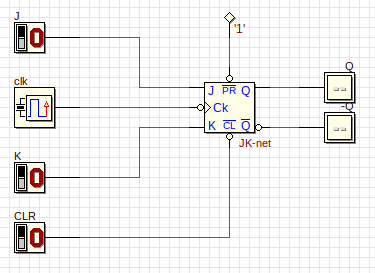
\includegraphics[width=0.5\textwidth]{Exp09/images/2.1.1.png}
  \caption{Implementação de um Flip-Flop JK-Net utilizando Deeds 3}\label{fig:2.1.1.png}
\end{figure}

Deve atentar-se que este flip-flop depende de sua borda de descida para a
mudança de estados.
\\
Simulando tem-se que seu diagrama de ondas será:

\begin{figure}[H]
  \centering
  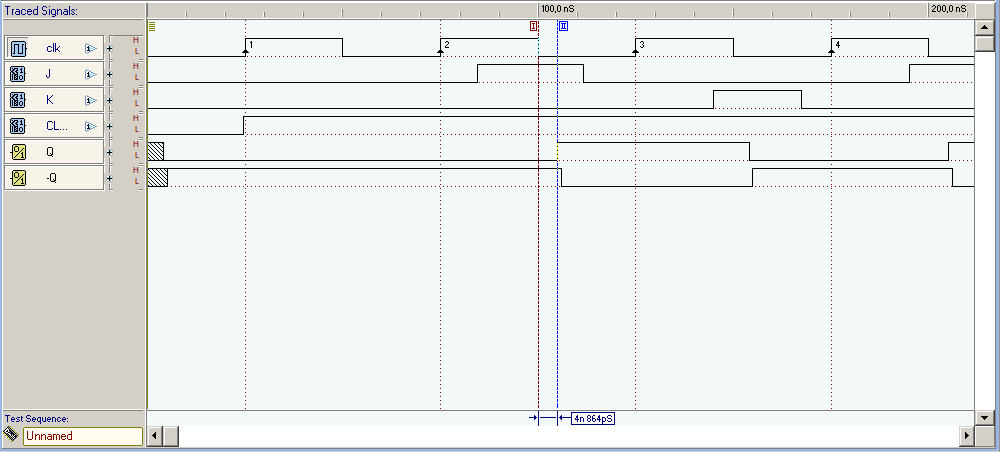
\includegraphics[width=1.0\textwidth]{Exp09/images/2.1.2.png}
  \caption{Diagrama de Onda de um Flip-Flop JK-Net}\label{fig:2.1.2.png}
\end{figure}
\href{}{}

Observa-se que também realizou-se uma medida de atraso em sua saída, sendo então de aproximadamente $4,864nS$.

Portando, observa-se que:

\begin{equation}
t_{co}\approx4,864nS
\end{equation}

Para um contador de 4 estágios tem-se que a máxima frequência será determinada por:

\begin{align}
f_{\max} &= \frac{1}{N.t_{co}}\\
f_{\max} &= \frac{1}{4.t_{co}}\\
f_{\max} &= \frac{1}{4.(4,864nS)}\\
f_{\max} &\approx51Mhz
\end{align}

Para um contador com frequência de $18Mhz$ e o tempo de atraso de $t_{co}$, então o número máximo de estágios será:

\begin{align}
f_{\max} &= \frac{1}{N.t_{co}}\\
N &= \frac{1}{f_{\max}.t_{co}}\\
N &= \frac{1}{18.10^{6}.(4,864.10^{-9})}\\
N &= \frac{1}{18.4,864.10^{-3}}\\
N &\approx11
\end{align}

Neste caso realiza-se um arredondamento para baixo, caso contrário será um número acima do esperado.

% 2.2
\subsection{Implementação de um Contador Binário Progressivo Assíncrono}\label{sec:2.2}

O circuito implementado será:
\begin{figure}[H]
  \centering
  \includegraphics[width=1.0\textwidth]{Exp09/images/2.2.1.png}
  \caption{Contador 4 Estágios}\label{fig:2.2.1.png}
\end{figure}

Simulando teremos então:
\href{google.com}{Linkzão Maroto}
\\
Para a simulação de onda em um clock de $5Mhz$ deste mesmo circuito teremos:
\begin{figure}[H]
  \centering
  \includegraphics[width=1.1\textwidth]{Exp09/images/2.2.2.png}
  \caption{Diagrama de Ondas de um Contador 4 Estágios}\label{fig:2.2.2.png}
\end{figure}

Fator a ser mencionado é o fato de que existem certos glitches em $C_{0}$, sendo assim, temos que em algumas de suas transições momentaneamente o valor de saída não é o esperado, 
parte dos momentos em que tal erro ocorre são quando $C_{0}=0$, ou seja, todas as saídas utilizadas resultam em 0.\\ \\
Assim, sua tabela será definida por:
\begin{table}[H]
    \centering
    \caption{Tabela Verdade para \emph{Contador Assíncrono 4 Estágios}}
    \begin{tabular}{|c|c|c|c|c|c|c|c|}\hline
      \multicolumn{4}{|c|}{Estado Atual} & \multicolumn{4}{|c|}{Próximo Estado} \\\hline
      \textbf{$Q_{3}$} & \textbf{$Q_{1}$} & \textbf{$Q_{2}$} & \textbf{$Q_{0}$} & \textbf{$Q_{3}$} & \textbf{$Q_{2}$} & \textbf{$Q_{1}$} & \textbf{$Q_{0}$} \\\hline
      0 & 0 & 0 & 0 & 0 & 0 & 0 & 1 \\\hline
      0 & 0 & 0 & 1 & 0 & 0 & 1 & 0 \\\hline
      0 & 0 & 1 & 0 & 0 & 0 & 1 & 1 \\\hline
      0 & 0 & 1 & 1 & 0 & 1 & 0 & 0 \\\hline
      0 & 1 & 0 & 0 & 0 & 1 & 0 & 1 \\\hline
      0 & 1 & 0 & 1 & 0 & 1 & 1 & 0 \\\hline
      0 & 1 & 1 & 0 & 0 & 1 & 1 & 1 \\\hline
      0 & 1 & 1 & 1 & 1 & 0 & 0 & 0 \\\hline
      1 & 0 & 0 & 0 & 1 & 0 & 0 & 1 \\\hline
      1 & 0 & 0 & 1 & 1 & 0 & 1 & 0 \\\hline
      1 & 0 & 1 & 0 & 1 & 0 & 1 & 1 \\\hline
      1 & 0 & 1 & 1 & 1 & 1 & 0 & 0 \\\hline
      1 & 1 & 0 & 0 & 1 & 1 & 0 & 1 \\\hline
      1 & 1 & 0 & 1 & 1 & 1 & 1 & 0 \\\hline
      1 & 1 & 1 & 0 & 1 & 1 & 1 & 1 \\\hline
      1 & 1 & 1 & 1 & 0 & 0 & 0 & 0 \\\hline
    \end{tabular}\label{tab:truth_table_latch_rs_triggered}
\end{table}

Adotando para este mesmo circuito um clock de $53.63MHz$, tem-se que seu diagrama será descrito por:
\begin{figure}[H]
  \centering
  \includegraphics[width=1.1\textwidth]{Exp09/images/2.2.4.1.png}
  \caption{Diagrama de Ondas de um Contador 4 Estágios com clock de }\label{2.2.4.1.png}
\end{figure}

\begin{figure}[H]
  \centering
  \includegraphics[width=1.1\textwidth]{Exp09/images/2.2.4.1.png}
  \caption{Diagrama de Ondas de um Contador 4 Estágios com clock de }\label{2.2.4.1.png}
\end{figure}

Com os resultados obtidos observa-se então que os valores não seguem sua contagem padrão, apresentando comportamento irregular pelo fato da alta frequência não criar tempo necessário para descrever as mudanças.

% 2.3
\subsection{Implementação de um Contador em Anel}\label{sec:2.3}

Para esse tópico precisamos projetar e, posteriormente, desenhar no \emph{Deeds}
um circuito que opere como contador em anel de $4$ estágios.

Começaremos, portanto, projetando o circuito. Como ensinado
em~\cite{circuito_anel_CL}, podemos criar um contador em anel acoplando vários
\emph{Flip-Flops JK} em série, assim como mostrado na
imagem~\ref{fig:2.1.3_circuit.png}.

\begin{figure}[H]
  \centering
  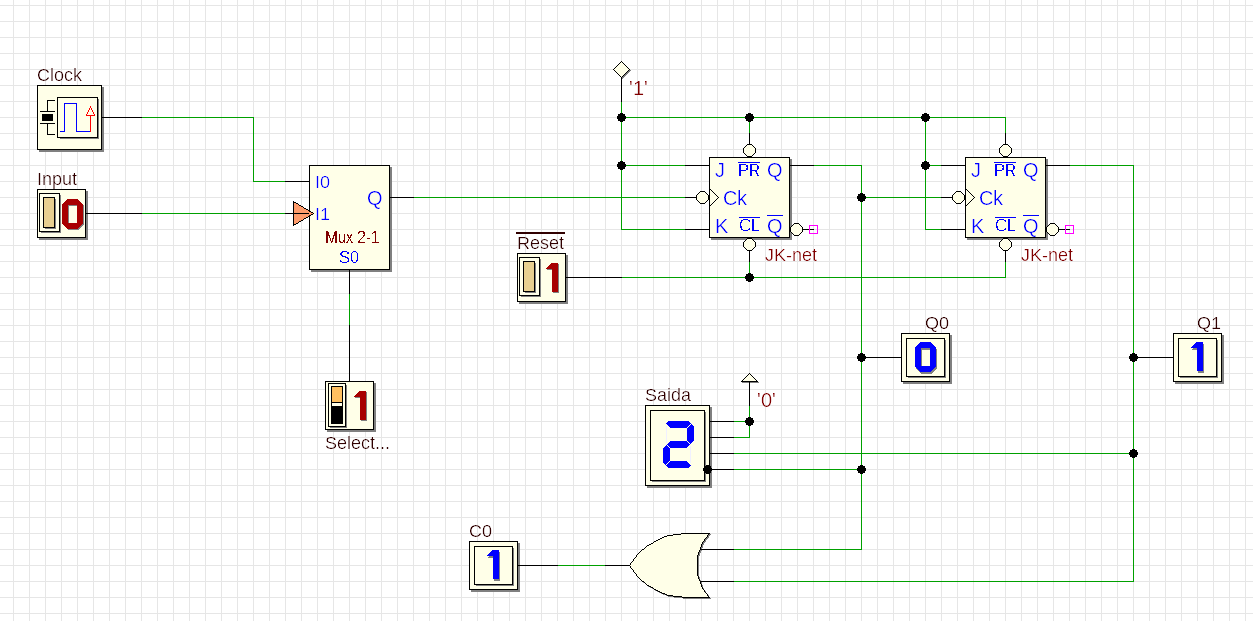
\includegraphics[width=0.7\textwidth]{Exp09/images/2.1.3_circuit.png}
  \caption{Circuito para o contador em anel de 4 estágios}\label{fig:2.1.3_circuit.png}
\end{figure}

Assim, nós dispomos agora do circuito requisitado para este tópico. O próximo
passo agora é a demonstração do circuito operando. Para isso, confira no vídeo a
seguir a simulação interativa no \emph{Deeds}:
\href{https://youtu.be/ylULsK-WZhA}{https://youtu.be/ylULsK-WZhA}

Por fim, faremos a análise da simulação em forma de onda para esse circuito.
Como é possível verificar na figura~\ref{fig:2.1.3.wave.1.png}, o circuito
possui dois estados transitórios significativos, que são os estágios
``$1 \rightarrow 2$'' e ``$3 \rightarrow 0$''.

Medindo os intervalos, podemos ver pelas figuras~\ref{fig:2.1.3.wave.2.1.png}
e~\ref{fig:2.1.3.wave.2.2.png} que o intervalos ``$1 \rightarrow 2$'' e
``$3 \rightarrow 0$'' são de respectivamente $5nS$ e $4nS$.

\begin{figure}[H]
  \centering
  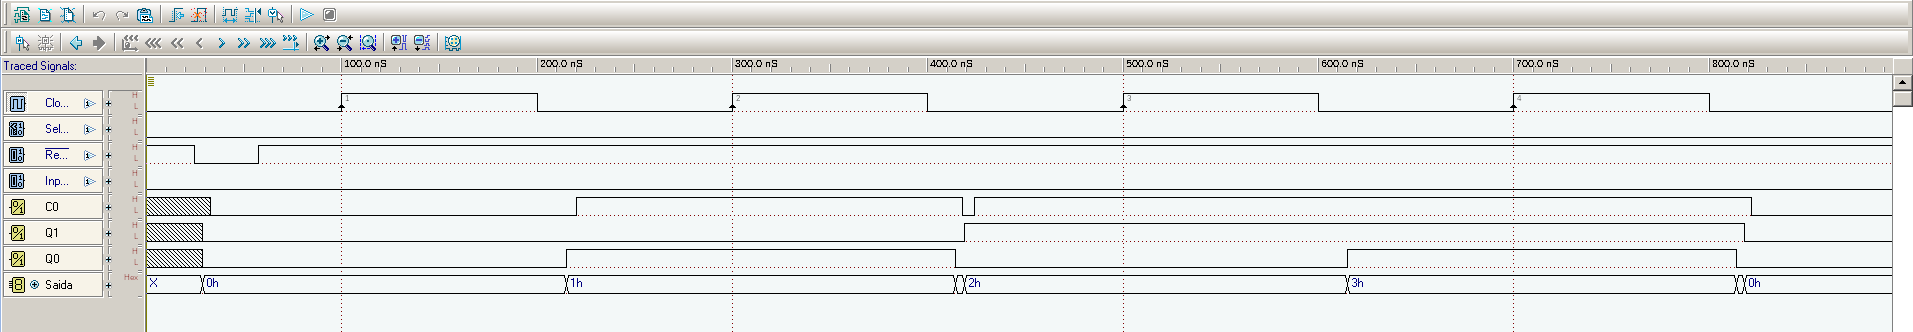
\includegraphics[width=1\textwidth]{Exp09/images/2.1.3.wave.1.png}
  \caption{Simulação em forma de onda}\label{fig:2.1.3.wave.1.png}
\end{figure}

\begin{figure}[H]
  \centering
  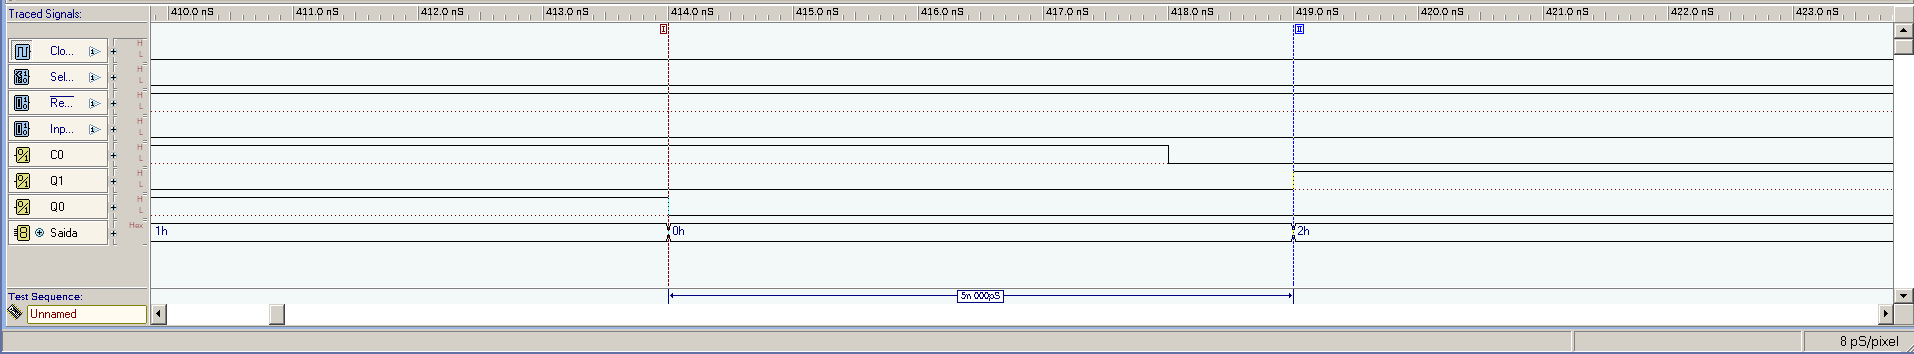
\includegraphics[width=1\textwidth]{Exp09/images/2.1.3.wave.2.1.png}
  \caption{Zoom na transição $1 \rightarrow 2$}\label{fig:2.1.3.wave.2.1.png}
\end{figure}

\begin{figure}[H]
  \centering
  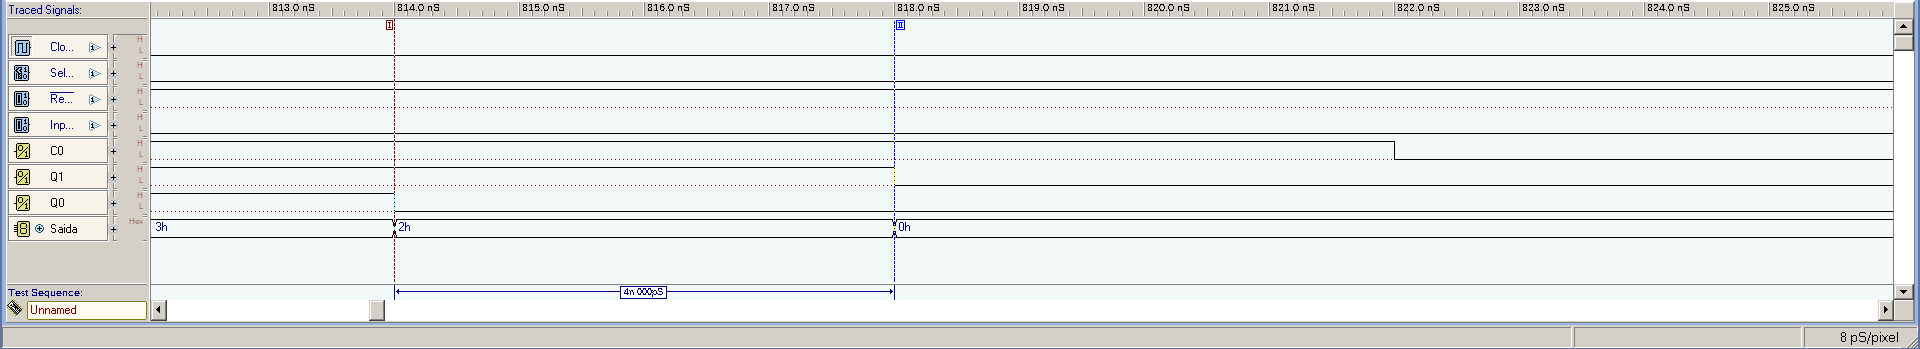
\includegraphics[width=1\textwidth]{Exp09/images/2.1.3.wave.2.2.png}
  \caption{Zoom na transição $3 \rightarrow 0$}\label{fig:2.1.3.wave.2.2.png}
\end{figure}


% 2.4
\subsection{TODO: Insert name}\label{sec:2.4}

\textbf{TODO}\\
\textbf{TODO: LINK DA PARTE 1:}\\
\href{}{}
\textbf{TODO: LINK DA PARTE 2:}\\
\href{}{}
\textbf{TODO: LINK DA PARTE 3:}\\
\href{}{}

\section{Análise dos Resultados}\label{sec:resultados}

Passaremos a analisar individualmente cada um dos tópicos anteriores, levantando
observações pertinentes para cada um deles.

\subsection{Análise do tópico~\ref{sec:2.1}}\label{sec:analise2.1}

Os resultados obtidos no tópico \ref{sec:2.1} 

\subsection{Análise do tópico~\ref{sec:2.2}}\label{sec:analise2.2}

\textbf{TODO}

\subsection{Análise do tópico~\ref{sec:2.3}}\label{sec:analise2.3}

\textbf{TODO}

\subsection{Análise do tópico~\ref{sec:2.4}}\label{sec:analise2.4}

\textbf{TODO}

\section{Conclusão}\label{sec:Conclusao}

\textbf{TODO}

\bibliographystyle{sbc}
\bibliography{relatorio}  %Aqui é a definição do arquivo .bib a ser usado pelas referências


\newpage
% Colocar aqui apenas as respostas dos itens da Auto-Avaliação
\section*{Auto-Avaliação}

Respostas:

\begin{table}[H]
      \begin{tabular}{|c|c|} \hline
      \textbf{Questão} & \textbf{Resposta}\\
      \hline
      1   & - \\ \hline
      2   & - \\ \hline
      3   & - \\ \hline
      4   & - \\ \hline
      5   & - \\ \hline
      6   & - \\ \hline
      7   & - \\ \hline
      8   & - \\ \hline
      9   & - \\ \hline
      10  & - \\ \hline
      11  & - \\ \hline
      12  & - \\ \hline
      13  & - \\ \hline
      14  & - \\ \hline
      15  & - \\ \hline
      16  & - \\ \hline
      17  & - \\ \hline
      18  & - \\ \hline
      19  & - \\ \hline
      20  & - \\ \hline
      21  & - \\ \hline
      22  & - \\ \hline
      23  & - \\ \hline
      24  & - \\ \hline
      25  & - \\ \hline
      26  & - \\ \hline
      27  & - \\ \hline
      28  & - \\ \hline
      29  & - \\ \hline
      30  & - \\ \hline
      31  & - \\ \hline
      32  & - \\ \hline
      \end{tabular}
\end{table}



\end{document}
